\documentclass[10pt,a4paper]{article}

\usepackage[T1]{fontenc}
\usepackage{newtxtext}
\usepackage[scaled=0.94]{helvet}
\usepackage[protrusion=true,expansion=true]{microtype}
\usepackage[left=14mm,right=14mm,top=10mm,bottom=10mm]{geometry}
\usepackage{graphicx}
\usepackage{xcolor}
\usepackage{tabularx}
\usepackage{enumitem}
\usepackage{tikz}
\usetikzlibrary{arrows.meta,positioning,calc}

\definecolor{PitchNavy}{HTML}{071B58}
\definecolor{PitchTeal}{HTML}{35BFC8}
\definecolor{PitchInk}{HTML}{182234}
\definecolor{PitchMuted}{HTML}{5B6470}
\definecolor{PitchPale}{HTML}{EEF6F7}
\definecolor{PitchRule}{HTML}{D7DEE5}

\pagestyle{empty}
\setlength{\parindent}{0pt}
\setlength{\parskip}{3.0pt}
\setlength{\emergencystretch}{1.5em}
\setlist[itemize]{
  leftmargin=4.2mm,
  label=\raisebox{0.25ex}{\color{PitchTeal!75!PitchNavy}\rule{0.75mm}{0.75mm}},
  itemsep=2.4pt,
  topsep=2.5pt,
  parsep=0pt,
  partopsep=0pt
}

\newcommand{\displayfont}{\fontfamily{phv}\selectfont}
\DeclareRobustCommand{\sepmark}{%
  \raisebox{0.3ex}{\color{PitchTeal!70!PitchNavy}\rule{0.75mm}{0.75mm}}%
}
\newcommand{\eyebrow}[1]{%
  {\displayfont\bfseries\color{PitchTeal!70!PitchNavy}%
  \fontsize{7.8}{8.5}\selectfont\MakeUppercase{#1}}%
}
\newcommand{\messagehead}[1]{%
  {\displayfont\bfseries\color{PitchNavy}%
  \fontsize{13.2}{14.5}\selectfont #1\par}%
  \vspace{1.5mm}%
  {\color{PitchTeal}\rule{17mm}{1.15pt}}\par
  \vspace{1.8mm}%
}
\newcommand{\sidehead}[1]{%
  {\displayfont\bfseries\color{PitchNavy}%
  \fontsize{12.4}{13.5}\selectfont #1\par}%
}
\newcommand{\personlabel}[1]{%
  {\displayfont\bfseries\color{PitchTeal!65!PitchNavy}%
  \fontsize{8.2}{9.0}\selectfont\MakeUppercase{#1}}%
}
\newcommand{\softpanel}[1]{%
  \begingroup
  \setlength{\fboxsep}{3.8mm}%
  \colorbox{PitchPale}{\parbox{\dimexpr\linewidth-2\fboxsep\relax}{#1}}%
  \endgroup
}

\begin{document}
\color{PitchInk}
\fontsize{9.6}{11.4}\selectfont
\raggedright

% Institutional row
\begin{tabularx}{\linewidth}{@{}>{\raggedright\arraybackslash}p{0.28\linewidth}>{\centering\arraybackslash}X>{\raggedleft\arraybackslash}p{0.20\linewidth}@{}}
  
\includegraphics[height=12.2mm]{../../assets/institutions/university-of-glasgow.png} &
  
\includegraphics[height=8.0mm]{../../assets/institutions/cuhk.png} &
  
\includegraphics[height=13.2mm]{../../assets/institutions/uestc.png}
\end{tabularx}

\vspace{2.3mm}
{\color{PitchRule}\rule{\linewidth}{0.55pt}}
\vspace{2.2mm}

\eyebrow{BMEG3920 \sepmark\ One-page pitch}

\vspace{1.5mm}
{\displayfont\bfseries\color{PitchNavy}\fontsize{29}{30.5}\selectfont LiteRehab Fusion}\par
\vspace{1.4mm}
{\displayfont\color{PitchMuted}\fontsize{11.7}{13.2}\selectfont
Immediate feedback for upper-limb rehabilitation practice at home.}\par

\vspace{4.2mm}
{\color{PitchTeal}\rule{\linewidth}{1.4pt}}
\vspace{4.2mm}

% Asymmetric body grid
\begin{minipage}[t]{0.625\linewidth}
  \vspace{0pt}
  \messagehead{Feedback arrives too late}
  A patient may leave a physiotherapy appointment knowing what to practise.
  At home, it is harder to tell whether the movement was controlled and large
  enough, or whether leaning did part of the work. By the next appointment,
  those repetitions are already behind them.

  \vspace{5.5mm}
  \messagehead{LiteRehab responds during the repetition}
  LiteRehab gives a cue while the exercise is still happening. A forearm
  wearable tracks motion, while a camera checks posture. Together, they
  identify the demonstrated exercise, count repetitions, and flag excessive
  speed, limited range, or trunk compensation. The dashboard also keeps a
  synchronized session record.

  \vspace{6.2mm}
  \messagehead{Motion and posture, seen together}

  \begin{center}
  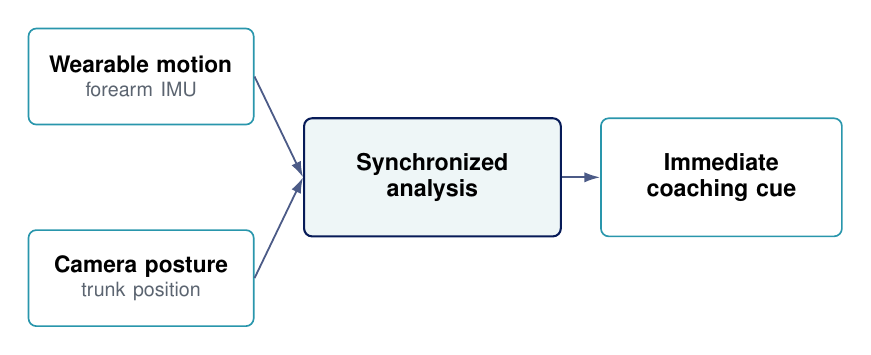
\begin{tikzpicture}[
    input/.style={
      draw=PitchTeal!75!PitchNavy,
      fill=white,
      rounded corners=1mm,
      line width=0.6pt,
      minimum height=12.2mm,
      text width=25mm,
      align=center,
      inner sep=1.8mm,
      font=\displayfont\fontsize{8.2}{9.2}\selectfont
    },
    core/.style={
      draw=PitchNavy,
      fill=PitchPale,
      rounded corners=1mm,
      line width=0.75pt,
      minimum height=15mm,
      text width=29mm,
      align=center,
      inner sep=1.8mm,
      font=\displayfont\bfseries\fontsize{8.4}{9.4}\selectfont
    },
    output/.style={
      draw=PitchTeal!75!PitchNavy,
      fill=white,
      rounded corners=1mm,
      line width=0.6pt,
      minimum height=15mm,
      text width=27mm,
      align=center,
      inner sep=1.8mm,
      font=\displayfont\bfseries\fontsize{8.4}{9.4}\selectfont
    },
    flow/.style={
      -{Latex[length=2.0mm,width=1.3mm]},
      draw=PitchNavy!72,
      line width=0.65pt
    }
  ]
    \node[input] (motion) at (1.35,1.28) {\textbf{Wearable motion}\\[-0.2mm]{\color{PitchMuted}\fontsize{7.1}{7.8}\selectfont forearm IMU}};
    \node[input] (posture) at (1.35,-1.28) {\textbf{Camera posture}\\[-0.2mm]{\color{PitchMuted}\fontsize{7.1}{7.8}\selectfont trunk position}};
    \node[core] (analysis) at (5.05,0) {Synchronized\\analysis};
    \node[output] (cue) at (8.72,0) {Immediate\\coaching cue};

    \draw[flow] (motion.east) -- (analysis.west);
    \draw[flow] (posture.east) -- (analysis.west);
    \draw[flow] (analysis.east) -- (cue.west);
  \end{tikzpicture}
  \end{center}

  \vspace{1.0mm}
  \begingroup
  \setlength{\fboxsep}{2.8mm}
  \colorbox{PitchPale}{%
    \parbox{\dimexpr\linewidth-2\fboxsep\relax}{%
      \centering\displayfont\color{PitchNavy}\fontsize{8.6}{10.0}\selectfont
      ``Slow down''\quad\sepmark\quad
      ``Increase the range''\quad\sepmark\quad
      ``Keep the trunk still''
    }%
  }
  \endgroup

  \vspace{2.7mm}
  {\displayfont\color{PitchMuted}\fontsize{7.8}{9.0}\selectfont
  Forearm wearable (MPU6050 + ESP32) \sepmark\ BLE receiver
  \sepmark\ MaixCAM2 posture stream \sepmark\ computer dashboard}

  \vspace{7.2mm}
  \messagehead{The wearable sees movement. The camera sees posture.}

  \begin{tabularx}{\linewidth}{@{}>{\raggedright\arraybackslash}X@{\hspace{6mm}}>{\raggedright\arraybackslash}X@{}}
    {\color{PitchTeal}\rule{18mm}{0.9pt}}\par
    \vspace{1.2mm}
    \personlabel{Wearable motion}\par
    \vspace{1.0mm}
    Repetition timing and movement range from the forearm.
    &
    {\color{PitchTeal}\rule{18mm}{0.9pt}}\par
    \vspace{1.2mm}
    \personlabel{Camera posture}\par
    \vspace{1.0mm}
    A wider view that can flag trunk compensation.
  \end{tabularx}
\end{minipage}
\hfill
\begin{minipage}[t]{0.34\linewidth}
  \vspace{0pt}\raggedright
  \softpanel{%
    \raggedright
    \eyebrow{Working prototype}\par
    \vspace{2.0mm}
    \sidehead{What the prototype\\does today}
    \vspace{2.2mm}
    \begin{itemize}
      \item Recognises the demonstrated elbow flexion and forearm rotation exercises.
      \item Gives feedback for excessive speed, insufficient range, and trunk compensation.
      \item Shows the repetition count and records synchronized motion and posture data.
      \item Uses a classroom CNN-BiGRU baseline with a rule-based fallback.
    \end{itemize}
  }

  \vspace{8.0mm}
  \sidehead{A cue now, a record for later}
  \vspace{2.2mm}
  {\color{PitchTeal}\rule{17mm}{1.15pt}}\par
  \vspace{2.8mm}
  \personlabel{For the person practising}\par
  \vspace{1.1mm}
  A short cue arrives in time to adjust the next repetition.

  \vspace{4.2mm}
  \personlabel{For the physiotherapist}\par
  \vspace{1.1mm}
  A session record could show what happened between appointments. Exercise
  selection and clinical decisions remain with the physiotherapist.

  \vspace{8.0mm}
  {\color{PitchTeal}\rule{\linewidth}{1.4pt}}\par
  \vspace{2.6mm}
  \sidehead{Next: supervised usability\\testing}
  \vspace{2.2mm}
  Our next step is to test the workflow with physiotherapists and representative
  users. Their feedback would help us refine the prompts and collect movement
  data under professional supervision.
\end{minipage}

\vspace{3.5mm}
{\color{PitchRule}\rule{\linewidth}{0.65pt}}\par
\vspace{1.8mm}
\eyebrow{Coursework prototype \sepmark\ Not a medical device}\par
\vspace{1.4mm}
{\color{PitchMuted}\fontsize{9.0}{10.2}\selectfont
LiteRehab Fusion does not diagnose, prescribe treatment, score recovery, or
replace professional supervision. The current system supports a limited
exercise set and makes no clinical accuracy claim.}

\end{document}
